\documentclass[tikz, margin=0mm]{standalone}

\usetikzlibrary{calc,patterns,positioning,arrows,arrows.meta,arrows.spaced,decorations.pathmorphing}

\def\centerarc[#1](#2)(#3:#4:#5);%
%Syntax: [draw options] (center) (initial angle:final angle:radius)
{
	\draw[#1,double distance=2mm]([shift=(#3:#5)]#2) arc (#3:#4:#5);
}

\makeatletter
\def\grd@save@target#1{%
	\def\grd@target{#1}}
\def\grd@save@start#1{%
	\def\grd@start{#1}}
\tikzset{
	grid with coordinates/.style={
		to path={%
			\pgfextra{%
				\edef\grd@@target{(\tikztotarget)}%
				\tikz@scan@one@point\grd@save@target\grd@@target\relax
				\edef\grd@@start{(\tikztostart)}%
				\tikz@scan@one@point\grd@save@start\grd@@start\relax
				\draw[minor help lines] (\tikztostart) grid (\tikztotarget);
				\draw[major help lines] (\tikztostart) grid (\tikztotarget);
				\grd@start
				\pgfmathsetmacro{\grd@xa}{\the\pgf@x/1cm}
				\pgfmathsetmacro{\grd@ya}{\the\pgf@y/1cm}
				\grd@target
				\pgfmathsetmacro{\grd@xb}{\the\pgf@x/1cm}
				\pgfmathsetmacro{\grd@yb}{\the\pgf@y/1cm}
				\pgfmathsetmacro{\grd@xc}{\grd@xa + \pgfkeysvalueof{/tikz/grid with coordinates/major step}}
				\pgfmathsetmacro{\grd@yc}{\grd@ya + \pgfkeysvalueof{/tikz/grid with coordinates/major step}}
				\foreach \x in {\grd@xa,\grd@xc,...,\grd@xb}
				\node[anchor=north] at (\x,\grd@ya) {\pgfmathprintnumber{\x}};
				\foreach \y in {\grd@ya,\grd@yc,...,\grd@yb}
				\node[anchor=east] at (\grd@xa,\y) {\pgfmathprintnumber{\y}};
			}
		}
	},
	minor help lines/.style={
		help lines,
		step=\pgfkeysvalueof{/tikz/grid with coordinates/minor step}
	},
	major help lines/.style={
		help lines,
		line width=\pgfkeysvalueof{/tikz/grid with coordinates/major line width},
		step=\pgfkeysvalueof{/tikz/grid with coordinates/major step}
	},
	grid with coordinates/.cd,
	minor step/.initial=.2,
	major step/.initial=1,
	major line width/.initial=0.1mm,
}
\makeatother
\begin{document}
\begin{tikzpicture}[decoration={random steps,segment length=1mm,amplitude=0.3mm}]
	
	\node at (0,0){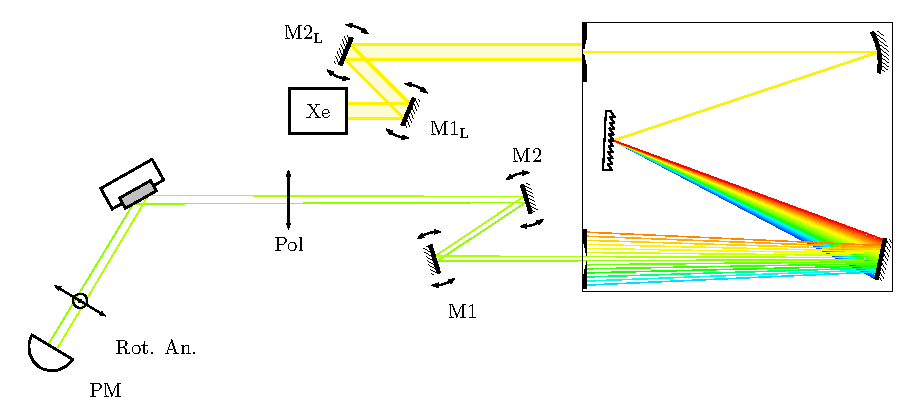
\includegraphics{build/SE-SETUP}};



%\draw [help lines](-8,-4) grid (8,4);

%\draw (-8,-4) to[grid with coordinates] (8,4);


 
% \filldraw[color=red!60, fill=red!5, very thick,opacity=0.3](-4.2,0.2) circle (1.5);
 % \filldraw[color=red!60, fill=red!5, very thick,opacity=0.3](-4.2,0.2) circle (1.35);
  
  
%  \draw [blue] (-2.7,0.2) arc [radius=1.5, start angle=0, end angle=60];
%  \draw [blue] (-3.9,1.65) arc [radius=1.2, start angle=75, end angle=108];
%  \draw [blue] (-5,1.5) arc [radius=1.65, start angle=125, end angle=180];
%  \draw [blue] (-5.68,-0.1) arc [radius=1.5, start angle=192, end angle=230];
%  \draw [blue] (-4.8,-1.2) arc [radius=1.5, start angle=247, end angle=285];
%   \draw [blue] (-3.5,-1.12) arc [radius=1.5, start angle=297, end angle=345];
%   

\centerarc[thick,decorate,double=gray!20](-5.5,0.2)(7:60:1.5cm);
%\centerarc[thick,decorate,gray](-5.5,0.2)(3:60:1.3cm);


\centerarc[thick,decorate,double=gray!20](-5.5,0.2)(75:110:1.5cm);
%\centerarc[thick,decorate,gray](-5.5,0.2)(75:110:1.3cm);

\centerarc[thick,decorate,double=gray!20](-5.5,0.2)(120:180:1.5cm);
%\centerarc[thick,decorate,gray](-5.5,0.2)(120:180:1.3cm);

\centerarc[thick,decorate,double=gray!20](-5.5,0.2)(190:230:1.5cm);
%\centerarc[thick,decorate,gray](-5.5,0.2)(190:230:1.3cm);

\centerarc[thick,decorate,double=gray!20](-5.5,0.2)(250:290:1.5cm);
%\centerarc[thick,decorate,gray](-5.5,0.2)(250:290:1.3cm);

\centerarc[thick,decorate,double=gray!20](-5.5,0.2)(300:345:1.5cm);
%\centerarc[thick,decorate,gray](-5.5,0.2)(300:345:1.3cm);

\draw[decorate,double=gray!20] (-6,1.6)--(-7,4);
\draw[decorate,double=gray!20] (-6.2,1.4)--(-7.3,3.9);


\draw[<->] (-5.6,-0.4) arc(270:330:1);

\node[scale=1.2] at(-5,-0.5){$\theta$}; 
%\draw[decorate,double=gray!10,double distance=4mm] (-5,1.3)--(-4.7,2.1);
%\draw[decorate,double=gray!10,double distance=4mm,opacity=0.3] (-4.3,-0)--(-3.5,0);
\end{tikzpicture}


\end{document}